\section{Login-Page}
\label{login-page}

Existiert bereits ein Account ist es möglich sich über die Log In View mit diesem anzumelden. Dafür 
wir die Email als auch das Passwort benötigt. Hierzu wird wie auch beim \nameref{createAccount} eine 
simple HTML form verwendet. 

\begin{figure}[H]
    \begin{center}
      \frame{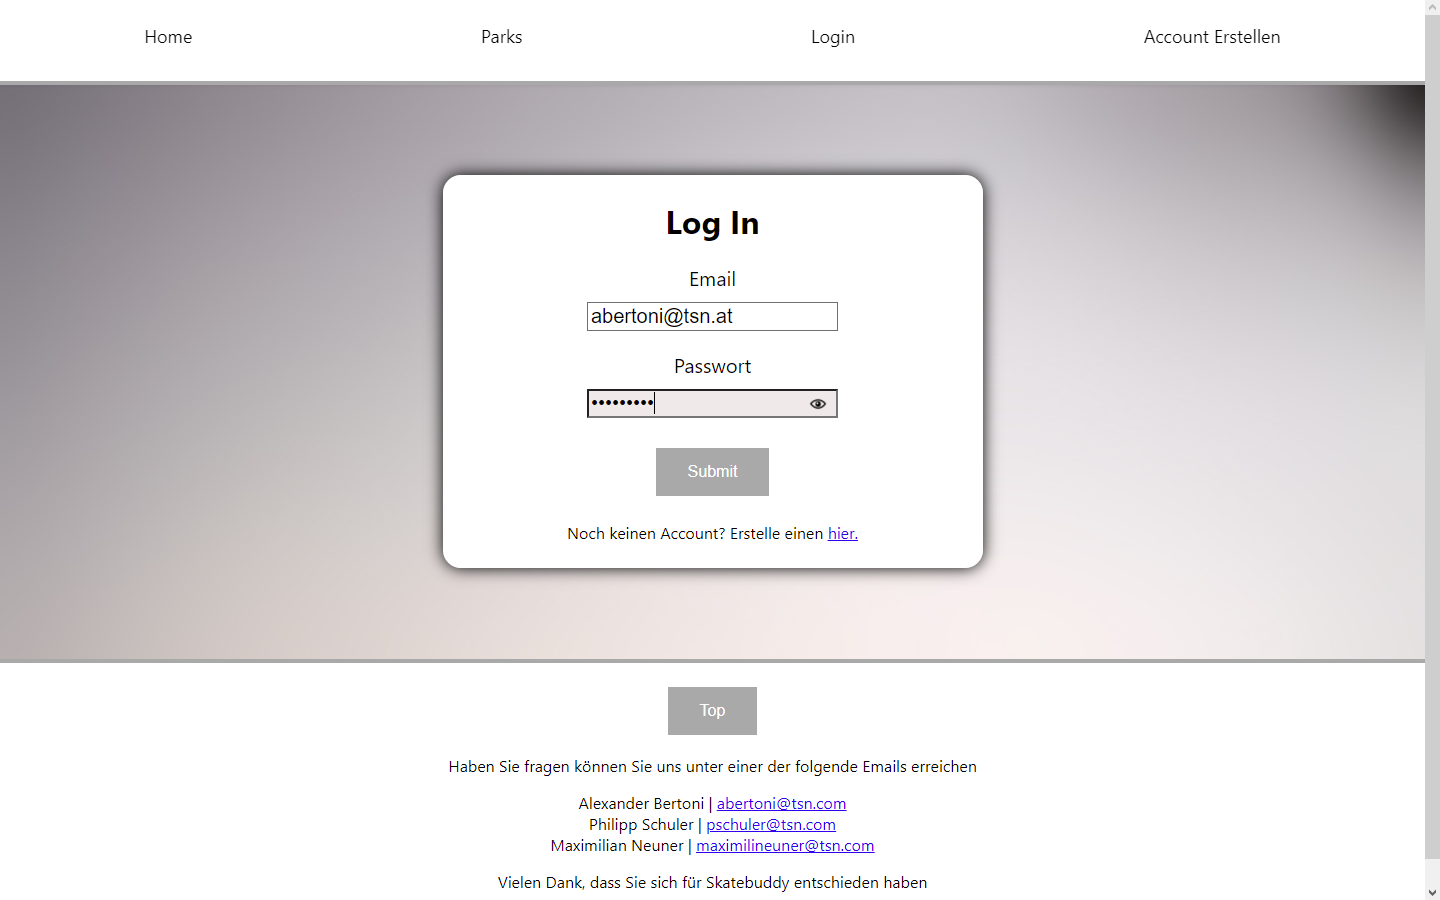
\includegraphics[width=1\textwidth]{Website/LogIn.png}}
      \caption{Login Page mit verstecktem Passwort}
    \end{center}
\end{figure}

Durch Mausklick auf das Auge in der Passwort Eingabe, lässt sich das Passwort für den Benutzer
anzeigen. Damit lassen sich Tippfehler beim Eingeben erkennen, falls nötig. 

\begin{figure}[H]
    \begin{center}
      \frame{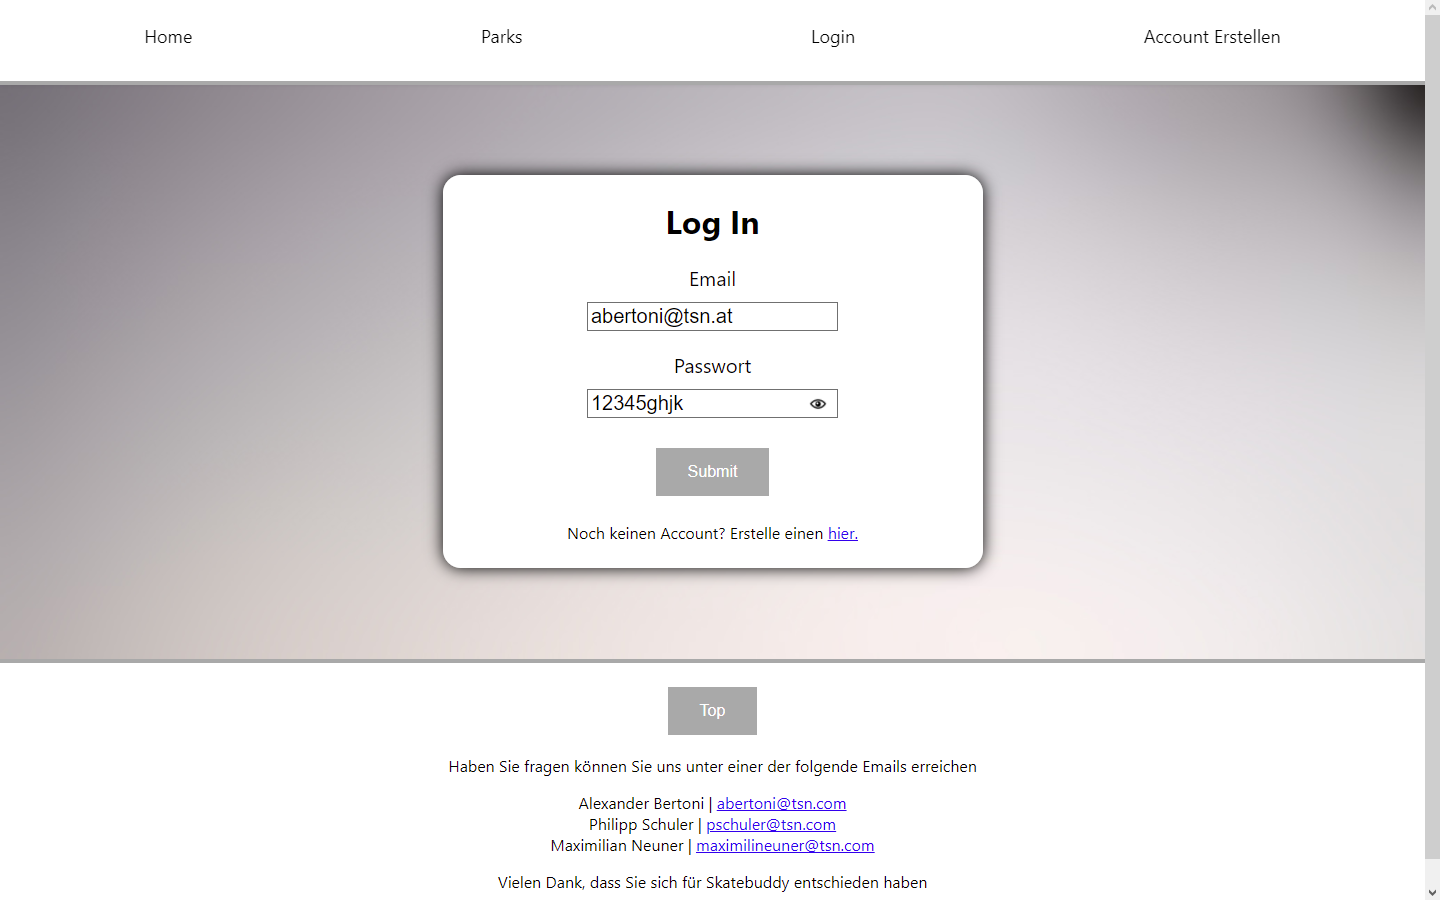
\includegraphics[width=1\textwidth]{Website/LogIn-Passwort-anzeigen.png}}
      \caption{Login Page mit gezeigtem Passwort}
    \end{center}
\end{figure}

\subsection{Augensymbol}

\begin{lstlisting}

    .toggle-button {
        margin-top: 0;
        margin-left: -30px;
        height: 17px;
        width: 20px;
        border: white;
        background: no-repeat url('./eye.png');
        background-size: cover;
        cursor: pointer;
    }

    const togglePassword = () =>{
        setPasswordShown(!passwordShown)
    }

    <input className="input" type={passwordShown ? "text" : "password"} onChange={e => setPassword(e.target.value)} />
    <button type="button" onClick={togglePassword} className="toggle-button"></button>
\end{lstlisting}


\label{login}